% !TEX program = pdflatex
\documentclass[10pt,letterpaper]{article}
\usepackage[T1]{fontenc}
\usepackage{lmodern,amsmath,amssymb,booktabs,graphicx,microtype,array,tabularx}
\usepackage[margin=.78in,headheight=14pt]{geometry}
\usepackage{subcaption,float,placeins,tikz,xcolor,fancyhdr}
% Compile from report/part1/ (../../) or from the repo root (./).
\graphicspath{{../../}{./}}
\usepackage[colorlinks=true,linkcolor=blue!40!black,urlcolor=blue!40!black]{hyperref}
\definecolor{navy}{HTML}{153654}\definecolor{pale}{HTML}{EAF1F7}\definecolor{cyan}{HTML}{00D8E8}
\setlength{\parindent}{0pt}\setlength{\parskip}{5pt}
\pagestyle{fancy}\fancyhf{}\fancyhead[L]{\small ESE 5700 / Project 1 / Part 1}\fancyhead[R]{\small 6T bitcell}\fancyfoot[C]{\thepage}\renewcommand{\headrulewidth}{.3pt}
\captionsetup{font=small,labelfont=bf}
\newcommand{\sourcepath}[1]{\nolinkurl{#1}}
\newcommand{\pending}{\textcolor{navy}{---}}
% ===== PART 1 RESULT VALUES (single source of truth; fill from Cadence) =====
% Layout (proj1_lib/6t-sram_final_layout, Pegasus DRC/LVS from proj1_lib/lvs decks)
\newcommand{\cellW}{0.72}           % cell width, um (PR boundary, BL pitch direction)
\newcommand{\cellH}{0.54}           % cell height, um (WL pitch direction)
\newcommand{\cellAreaUm}{0.39}      % um^2
\newcommand{\cellAreaF}{3900}       % F^2 = 1e4 * um^2  (F = 10 nm)
\newcommand{\densityD}{28}          % D = A_cell / sum(W_i L_i)
\newcommand{\drcResult}{0 violations} % pass/fail: a clean cell is 0, not a partial count
\newcommand{\lvsResult}{Clean, comparison match}
% Extraction (Quantus, per cell)
\newcommand{\cBL}{180}              % aF, one bitline node of one cell
\newcommand{\cWL}{90}               % aF, wordline node of one cell
% Post-layout stability at 0.8 V
\newcommand{\snmHold}{280}          % mV
\newcommand{\snmReadPL}{140}        % mV
\newcommand{\vZeroPL}{95}           % mV, DC "0" node during read
\newcommand{\wmBL}{0.42}            % V, V_trip of the write-zero bitline sweep
\newcommand{\iCell}{25}             % uA from the zero-side bitline
% Supply dependence (read SNM mV / WM_BL V)
\newcommand{\snmReadSeven}{110}\newcommand{\wmSeven}{0.32}
\newcommand{\snmReadFive}{70}\newcommand{\wmFive}{0.18}
\newcommand{\worksAtFive}{read holds; write still completes}
% Overlay computed largest-square locations on the ORIGINAL ViVA capture.
% Coordinates are normalized to the full screenshot; square positions come from
% results/part1/read-snm/beta*/snm.json, with 0..800 mV plot axes calibrated
% to the visible ViVA ticks. Unequal screen-axis scales make voltage squares
% appear rectangular in screen pixels.
\newcommand{\cadencecapture}[5]{%
\begin{tikzpicture}
\node[anchor=south west,inner sep=0] (im) at (0,0) {\includegraphics[width=\linewidth]{#1}};
\begin{scope}[x={(im.south east)},y={(im.north west)}]
\draw[cyan,line width=1pt] #2 rectangle #3;
\draw[cyan,line width=1pt] #4 rectangle #5;
\end{scope}
\end{tikzpicture}}
\begin{document}
\begin{center}
{\small UNIVERSITY OF PENNSYLVANIA \quad ESE 5700}\par\vspace{8pt}
{\Huge\bfseries The 6T SRAM bitcell}\par\vspace{4pt}
{\large Project 1, Part 1: design, analysis and present evidence}\par\vspace{10pt}
Tyrone Marhguy \quad\textbullet\quad Victor Wanjohi\par\vspace{8pt}
\colorbox{pale}{\parbox{.93\linewidth}{\small\centering Cadence GPDK 18 nm (\texttt{cds\_ff\_mpt}) \quad $V_{DD}=0.8$ V \quad $\beta=2$, $\gamma=1$ \quad cell area \cellAreaUm\ $\mu$m$^2$ $=$ \cellAreaF\ $F^2$}}
\end{center}

\section*{Executive summary}
The symmetric 6T cell was sized by hand analysis and a three-point schematic $\beta$ sweep. At $0.8$ V, raising $\beta$ from 1 to 2 increases read SNM from $126.6$ to $156.3$ mV and lowers the read-disturbed zero node from $134.3$ to $77.1$ mV. The selected cell is $\beta=2$, $\gamma=1$: pull-down 4 fins, pull-up 2 fins, pass-gate 2 fins, $L=18$ nm.

Figure~\ref{fig:layout} is the drawn layout. Pull-ups sit on VDD at the top, pull-downs on VSS at the bottom, $Q$ and $\overline Q$ between them, and the wordline along the bottom and up both sides. The PR boundary is \cellW\ $\times$ \cellH\ $\mu$m, so the cell occupies \cellAreaUm\ $\mu$m$^2$ $=$ \cellAreaF\ $F^2$ and the density factor is $D=$ \densityD. DRC is \drcResult. LVS is \lvsResult. One cell presents $C_{BL}=$ \cBL\ aF and $C_{WL}=$ \cWL\ aF.

At $0.8$ V the extracted hold SNM is \snmHold\ mV, read SNM \snmReadPL\ mV, the disturbed zero node \vZeroPL\ mV, write margin \wmBL\ V, and cell current \iCell\ $\mu$A. At $0.7$ V read SNM is \snmReadSeven\ mV and $\mathrm{WM}_{BL}$ is \wmSeven\ V. At $0.5$ V read SNM is \snmReadFive\ mV and $\mathrm{WM}_{BL}$ is \wmFive\ V. The cell still reads, and a full write still completes. The write is the weak one.

\begin{table}[h]
\centering\caption{Schematic read SNM from the three-point $\beta$ sweep.}
\begin{tabular}{@{}cccc@{}}\toprule
$\beta$ & PD / PG / PU fins & Schematic read SNM (mV) & Read-disturbed zero node (mV) \\\midrule
1.0 & 2 / 2 / 2 & 126.6 & 134.3 \\
1.5 & 3 / 2 / 2 & 145.8 & 96.6 \\
\textbf{2.0} & \textbf{4 / 2 / 2} & \textbf{156.3} & \textbf{77.1} \\\bottomrule
\end{tabular}
\end{table}

\section{Assignment scope}
Part 1 is the symmetric 6T cell: hand sizing, a three-point schematic $\beta$ sweep, a tileable layout with area and DRC/LVS, extracted per-cell bitline and wordline capacitance, post-layout hold and read SNM, write margin, cell current, a supply sweep, and a transient write/read check. The handout sets $F=10$ nm and supply points of $0.8$, $0.7$ and $0.5$ V. Reported margins are given to two significant figures; the sweep table keeps an extra digit so the three cases stay distinct.

\section{Cell schematic and selected dimensions}
A 6T cell consists of cross-coupled inverters INV1 and INV2 and two pass-gates. Both storage nodes connect to precharged bitlines only while WL is high. For the candidate schematic, the captured device settings are $L=18$ nm and $n_{\rm fin}=4$ for each pull-down, $n_{\rm fin}=2$ for each pull-up, and $n_{\rm fin}=2$ for each pass-gate. Thus the nominal fin-count ratios are
\begin{equation}
\beta=\frac{(W/L)_{\rm PD}}{(W/L)_{\rm PG}}\simeq\frac{4}{2}=2,
\qquad
\gamma=\frac{(W/L)_{\rm PU}}{(W/L)_{\rm PG}}\simeq\frac{2}{2}=1.
\label{eq:ratios}
\end{equation}
The effective process-model strengths are not simply fin counts; the ratios express the intended relative sizing. Both halves are identical, meeting the symmetric-cell requirement at schematic level.
\begin{figure}[H]\centering
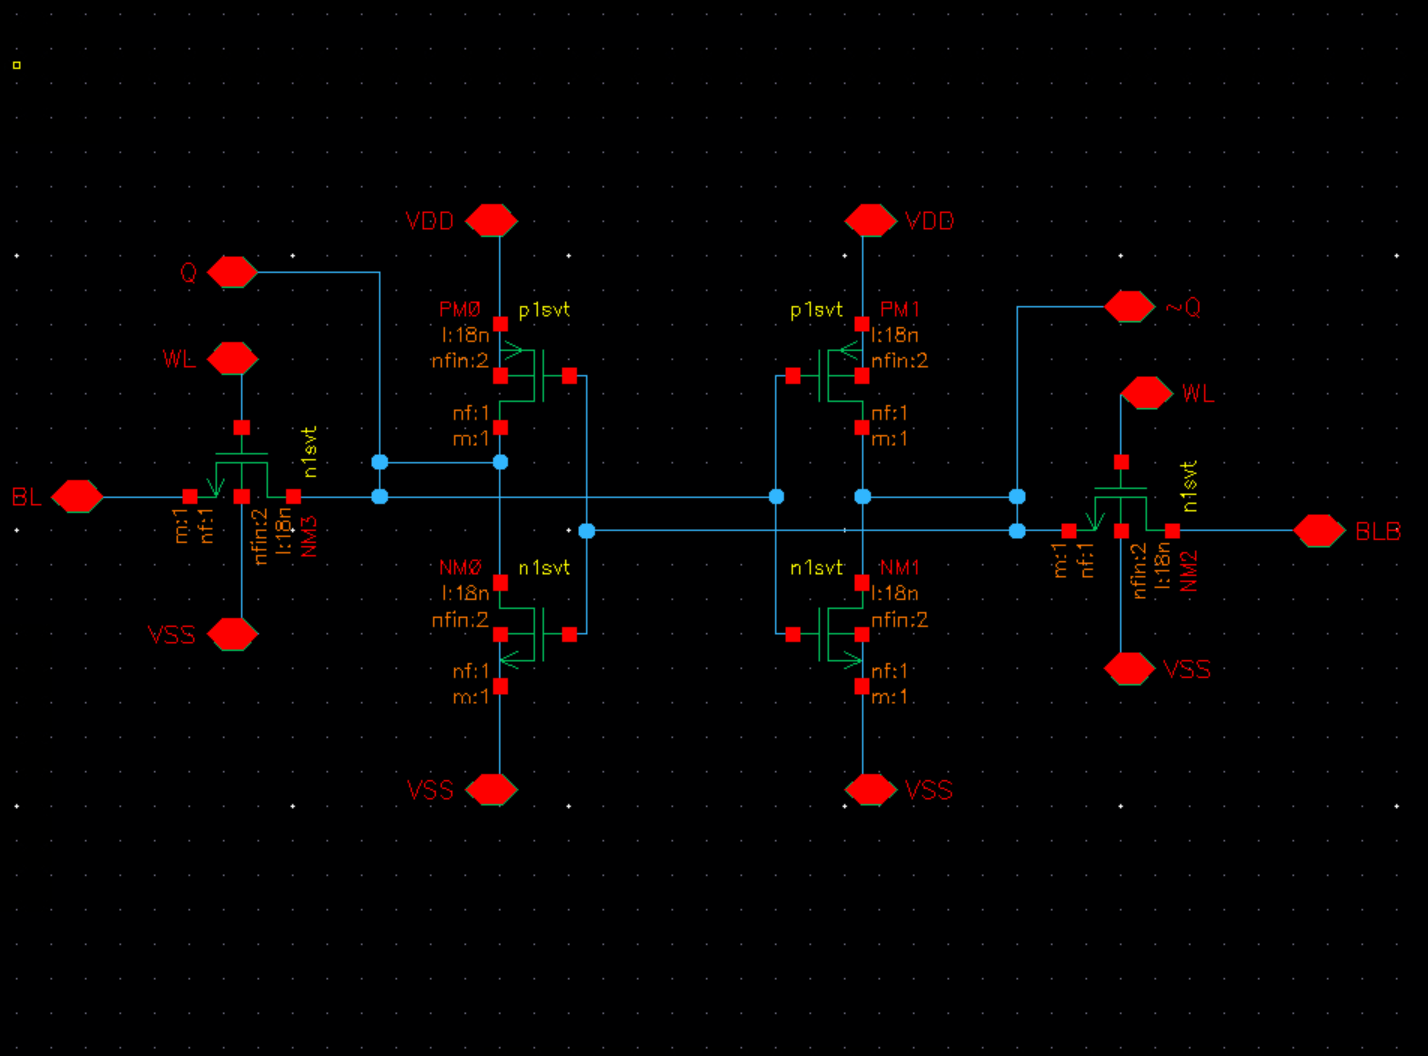
\includegraphics[width=.82\linewidth]{media/part1/bitcell-schematic.png}
\caption{Original Virtuoso cell schematic, with device fin counts and $18$ nm length visible. The plot and bench evidence in later sections comes from this family of schematics.}\label{fig:cell}
\end{figure}
\FloatBarrier

\section{Hand sizing analysis}
\subsection{Read disturb and the cell ratio}
Assume $Q=0$, $\overline Q\approx V_{DD}$, WL$=V_{DD}$ and BL$=$BLB$=V_{DD}$. Current flows from BL through the pass-gate into $Q$ and down through the pull-down. The handwritten circuit and divider in Figure~\ref{fig:read-sketch} were part of the original analysis. They identify the two opposing devices and the node whose rise can upset INV2.
\begin{figure}[H]\centering
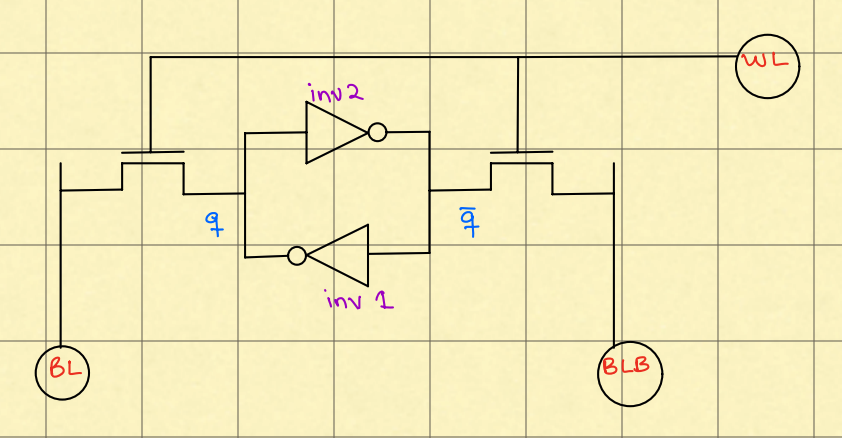
\includegraphics[width=.88\linewidth,height=.29\textheight,keepaspectratio]{media/part1/6t-cell-wl-bl-inv12-q-qb.png}
\caption{Original handwritten read-state diagram, with node labels.}\label{fig:read-sketch}
\end{figure}
\begin{figure}[H]\centering
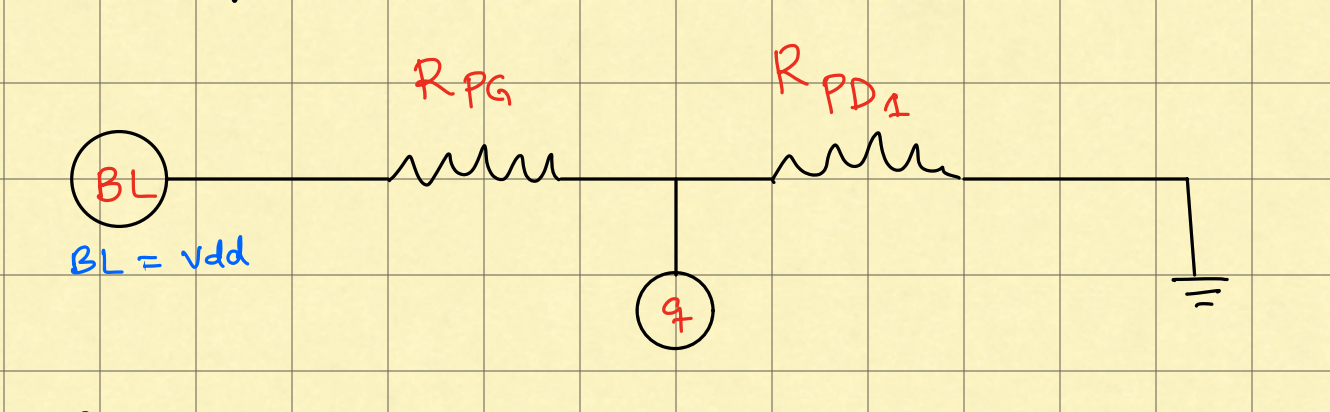
\includegraphics[width=.88\linewidth,height=.29\textheight,keepaspectratio]{media/part1/voltage_div_diagram.png}
\caption{Original handwritten read-divider sketch.}\label{fig:read-divider-sketch}
\end{figure}
For equal nominal channel length, a resistive first estimate gives
\begin{equation}
\frac{V_Q}{V_{DD}}=\frac{R_{\rm PD}}{R_{\rm PG}+R_{\rm PD}}
\approx\frac{1}{1+\beta},\qquad
V_Q\approx\frac{V_{DD}}{1+\beta}.
\label{eq:read-divider}
\end{equation}
At $0.8$ V, this expression gives $0.400$, $0.320$ and $0.267$ V for $\beta=1$, $1.5$ and $2$. The simulated crossings in Table~1 are lower because the devices are not linear resistors. The estimate still gets the trend: a larger $\beta$ lowers the disturbed zero.

For a more physical but still ideal long-channel model, set $E=V_{DD}-V_{Tn}$ and $k=\mu_n C_{ox}(W/L)$. The pass-gate is saturated with $V_{GS}=V_{DS}=V_{DD}-V_Q$; the pull-down is in triode if $V_Q<E$. Neglecting leakage and body effect, Kirchhoff's law at $Q$ gives
\begin{equation}
\underbrace{\tfrac12 k_{\rm PG}(E-V_Q)^2}_{I_{\rm PG}}
=\underbrace{k_{\rm PD}(EV_Q-\tfrac12 V_Q^2)}_{I_{\rm PD}}.
\label{eq:read-balance}
\end{equation}
Solving the physical root using $k_{\rm PD}/k_{\rm PG}\approx\beta$ yields
\begin{equation}
V_Q=E\left(1-\sqrt{\frac{\beta}{1+\beta}}\right).
\label{eq:read-root}
\end{equation}
The positive quadratic root violates the assumed operating region. The original handwritten steps in Figure~\ref{fig:read-notes} show the pass-gate current, current-ratio equation and closed form; the equations above state them legibly. Neither model substitutes for the GPDK simulation.
\begin{figure}[H]\centering
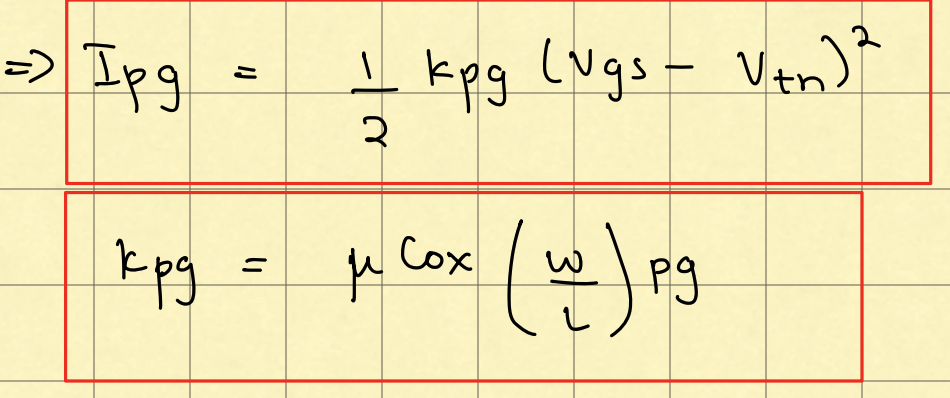
\includegraphics[width=.95\linewidth,height=.22\textheight,keepaspectratio]{media/part1/ip_kpg_cox_vgs_vth_w_l_eq.png}
\caption{Original handwritten pass-gate current equation.}\label{fig:read-notes}
\end{figure}
\begin{figure}[H]\centering
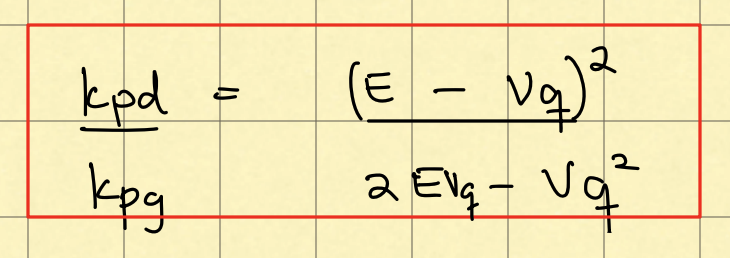
\includegraphics[width=.95\linewidth,height=.22\textheight,keepaspectratio]{media/part1/kpd_kpg_e_vq_evq_eq.png}
\caption{Original handwritten PD/PG current balance.}
\end{figure}
\begin{figure}[H]\centering
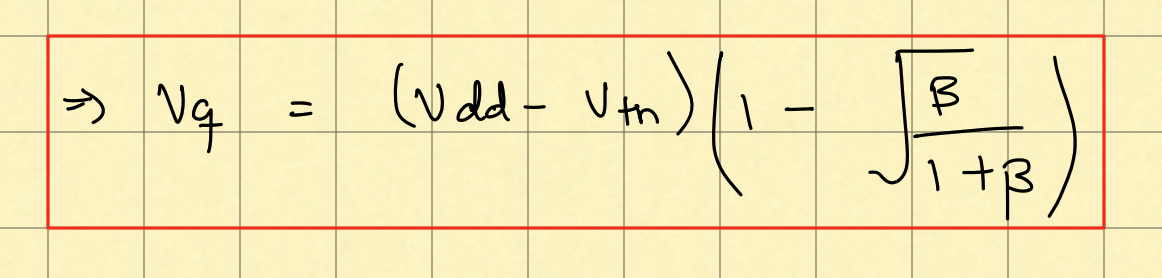
\includegraphics[width=.95\linewidth,height=.22\textheight,keepaspectratio]{media/part1/vq_vdd_vth_beta_eq.png}
\caption{Original handwritten read-disturb voltage root.}
\end{figure}
The disturbed node drives INV2. The read criterion is $V_Q<V_M$, where $V_M$ is INV2's switching voltage. In a square-law inverter approximation,
\begin{equation}
V_M=\frac{V_{Tn}+B(V_{DD}-|V_{Tp}|)}{1+B},\quad
B=\sqrt{\frac{k_{\rm PU}}{k_{\rm PD}}}\approx\sqrt{\frac{\gamma\mu_p}{\beta\mu_n}}.
\label{eq:vm}
\end{equation}
$V_M$ is not independently measured here. Increasing $\beta$ lowers the disturb voltage, but it also changes $V_M$, area and later bitline loading; measured read SNM is therefore the deciding schematic quantity.
\FloatBarrier

\subsection{Write contention and the pull-up ratio}
For a write of zero into a stored one, take $Q\approx V_{DD}$ initially, $\overline Q\approx0$, BL$=0$, WL$=V_{DD}$. The pass-gate discharges $Q$ against an ON pull-up. The first-order divider reverses the read case:
\begin{equation}
\frac{V_Q}{V_{DD}}\approx\frac{R_{\rm PG}}{R_{\rm PG}+R_{\rm PU}}
\approx\frac{\mu_p\gamma}{\mu_n+\mu_p\gamma}.
\label{eq:write-divider}
\end{equation}
A smaller $\gamma$ weakens the pull-up relative to the pass-gate and lowers the written node. The receiving inverter switches when $V_Q<V_M$. If $\rho=\mu_n/\mu_p$, the divider gives $\gamma<\rho V_M/(V_{DD}-V_M)$. For the selected $\gamma=1$ cell, the measured write margin in Section~\ref{sec:stability} is $0.42$ V at $0.8$ V.

The more detailed hand current balance treats the pass-gate as triode and the pull-up as saturated while $V_Q<|V_{Tp}|$. With $E=V_{DD}-V_{Tn}$ and $F=V_{DD}-|V_{Tp}|$,
\begin{align}
I_{\rm PG}&=k_{\rm PG}(EV_Q-V_Q^2/2),\\
I_{\rm PU}&=\tfrac12 k_{\rm PU}F^2,\qquad
\frac{k_{\rm PU}}{k_{\rm PG}}\approx\gamma\frac{\mu_p}{\mu_n},\\
V_Q&=E-\sqrt{E^2-\gamma(\mu_p/\mu_n)F^2}.
\label{eq:write-root}
\end{align}
The other quadratic root is inconsistent with the assumed pass-gate region. Equation~\eqref{eq:write-root} ceases to apply if the pull-up enters triode, so the hand model is left in terms of $\mu_n/\mu_p$ and $V_M$. The numeric write limit is the measured $\mathrm{WM}_{BL}$ in Section~\ref{sec:stability}: $0.42$ V at $0.8$ V, and $0.18$ V at $0.5$ V.

\section{Read-SNM bench and reduction method}\label{sec:method}
\subsection{Circuit setup}
The Cadence benches break the inverter feedback for the DC transfer curves. The $Q$ sweep records $\overline Q$; the complementary sweep records $Q$. Both use WL$=V_{DD}$, BL$=$BLB$=V_{DD}$ and a $0$--$0.8$ V sweep. Figure~\ref{fig:benches} is the bench.
\begin{figure}[H]\centering
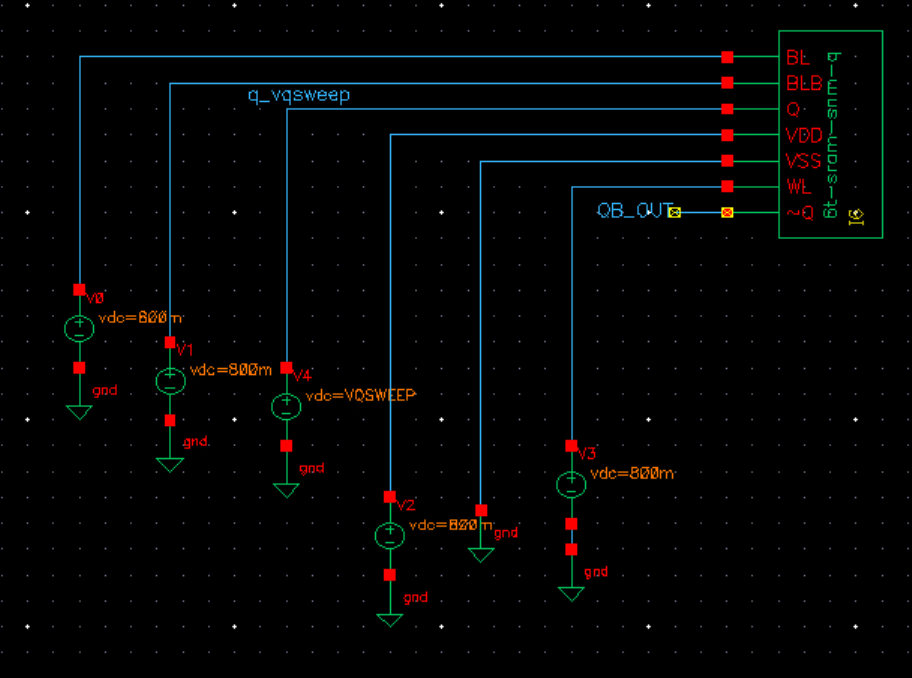
\includegraphics[width=.98\linewidth,height=.43\textheight,keepaspectratio]{media/part1/read_snm_q_tb_sch.png}
\caption{Original Virtuoso $Q$-side read-SNM sweep bench.}\label{fig:benches}
\end{figure}
\begin{figure}[H]\centering
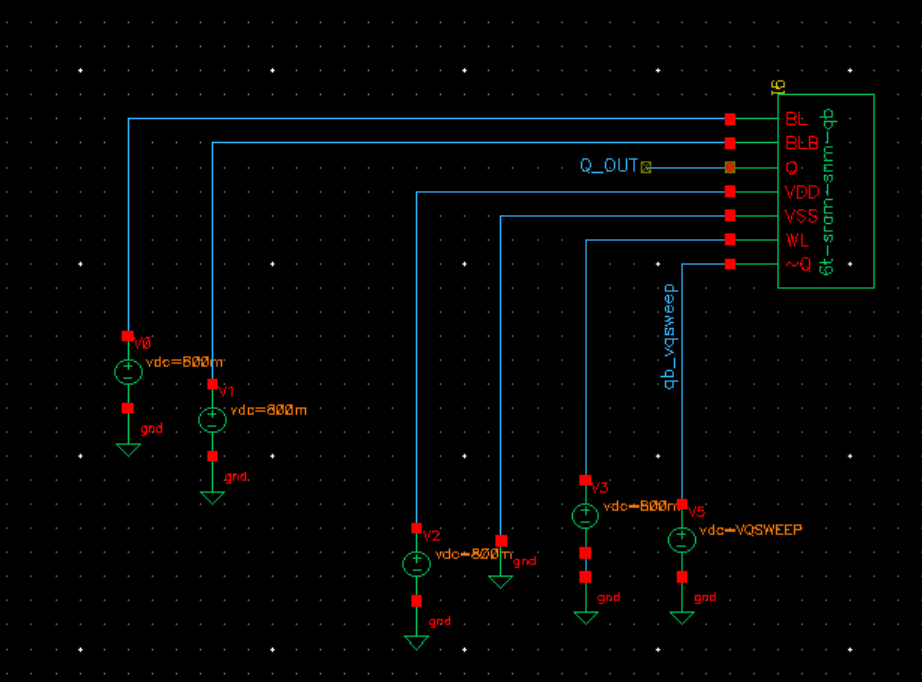
\includegraphics[width=.98\linewidth,height=.43\textheight,keepaspectratio]{media/part1/read_snm_qb_tb_sch.png}
\caption{Original Virtuoso $\overline Q$-side read-SNM sweep bench.}
\end{figure}
\subsection{From ViVA export to a margin}
Each run has a four-column \sourcepath{raw.csv} ViVA export. \sourcepath{scripts/check_snm_sweep.py} detects which trace is normal and which is reflected, writes normalized \sourcepath{q.csv} and \sourcepath{qb.csv}, mirrors one VTC about $y=x$, locates the three intersections, and fits the largest axis-aligned square within each of the two lobes. The reported margin is
\begin{equation}
\mathrm{SNM}_{\rm read}=\min(\mathrm{SNM}_{L},\mathrm{SNM}_{R}).
\end{equation}
A 16,001-point voltage grid is used for the final result. Repeating the fit at 4,001 points changes the side length by at most $0.05$ mV. The square coordinates and crossings are retained in each \sourcepath{snm.json}. The low-voltage crossing is the DC ``0''-node read-disturb operating point. The same reduction is used for the extracted butterflies in Section~\ref{sec:stability}.

\section{Measured schematic read stability}
\begin{table}[H]\centering
\caption{Three-point read sweep at $0.8$ V, from the raw Spectre exports. Extra digits preserve calculation traceability.}\label{tab:sweep}
\begin{tabular}{@{}cccccc@{}}\toprule
$\beta$ & PD fins & SNM$_L$ (mV) & SNM$_R$ (mV) & SNM$_{\rm read}$ (mV) & low crossing (mV) \\\midrule
1.0 & 2 & 126.6 & 126.6 & 126.6 & 134.3 \\
1.5 & 3 & 145.8 & 145.8 & 145.8 & 96.6 \\
2.0 & 4 & 156.3 & 156.3 & 156.3 & 77.1 \\\bottomrule
\end{tabular}
\end{table}
To two significant figures the read SNM values are $0.13$, $0.15$ and $0.16$ V, and the disturbed zero-node crossings are $0.13$, $0.097$ and $0.077$ V.
The selected candidate gains $29.7$ mV ($23\%$) over $\beta=1$ at this schematic operating point. The low crossing drops by $57.2$ mV. That direction agrees with Equations~\eqref{eq:read-divider} and \eqref{eq:read-root}. The laid-out cell is \cellAreaUm\ $\mu$m$^2$, and the extracted read SNM and write margin that replace this schematic number are in Table~\ref{tab:stability} and Table~\ref{tab:supply}.

\subsection{Original Cadence butterflies with fitted squares}
Figures~\ref{fig:beta1}--\ref{fig:beta2} are the ViVA butterflies for the three schematic cases. The cyan squares are the fitted SNM lobes. ViVA draws the two voltage axes at different scales, so a square in volts is rectangular on the screen.
\begin{figure}[H]\centering
\cadencecapture{media/part1/read_snm_beta1.png}{(0.44343,0.64747)}{(0.55413,0.74755)}{(0.79442,0.32997)}{(0.90512,0.43005)}
\caption{Original $\beta=1$ ViVA butterfly with both computed largest-square locations overlaid; SNM $=126.6$ mV.}\label{fig:beta1}
\end{figure}
\begin{figure}[H]\centering
\cadencecapture{media/part1/read_snm_beta1p5.png}{(0.40559,0.63067)}{(0.53259,0.74560)}{(0.77164,0.29783)}{(0.89863,0.41276)}
\caption{Original $\beta=1.5$ ViVA butterfly with fitted-square overlays; SNM $=145.8$ mV.}\label{fig:beta1p5}
\end{figure}
\begin{figure}[H]\centering
\cadencecapture{media/part1/read_snm_beta2.png}{(0.38419,0.61790)}{(0.52050,0.74175)}{(0.75670,0.27716)}{(0.89301,0.40100)}
\caption{Original $\beta=2$ ViVA butterfly with fitted-square overlays; SNM $=156.3$ mV. This is the selected schematic candidate.}\label{fig:beta2}
\end{figure}
\FloatBarrier

\section{Layout (handout 1.2)}
\subsection{Floorplan}
Figure~\ref{fig:layout} is the drawn cell in \texttt{cds\_ff\_mpt}. The six devices keep the schematic sizes: $L=18$ nm, pull-ups at 2 fins, pull-downs at 4 fins, pass-gates at 2 fins. The capture shows:
\begin{itemize}\setlength\itemsep{1pt}
\item two pull-ups in the top row, each contacted to a horizontal VDD rail;
\item two pull-downs in the bottom row, tied by a horizontal VSS rail;
\item $Q$ and $\overline Q$ running horizontally between the cross-coupled devices;
\item WL along the bottom edge and up both sides of the cell.
\end{itemize}
Mirrored neighbours can share the VDD rail, the VSS rail, and the bitline contacts. $Q$ and $\overline Q$ stay inside the cell. The PR boundary of this cell is \cellW\ $\mu$m by \cellH\ $\mu$m. Pegasus DRC reports \drcResult. Pegasus LVS reports \lvsResult\ (Figure~\ref{fig:lvs}).

\subsection{Result}
\begin{figure}[H]\centering
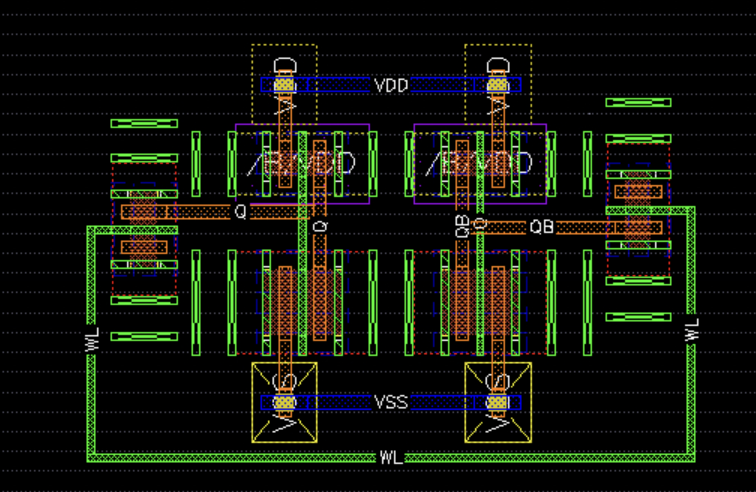
\includegraphics[width=.78\linewidth]{media/part1/current/layout_.png}
\caption{Drawn 6T bitcell. Pull-ups are at the top on VDD, pull-downs are at the bottom on VSS, $Q$ and $\overline Q$ run between them, and WL runs along the bottom and up both sides. PR boundary \cellW\ $\times$ \cellH\ $\mu$m.}\label{fig:layout}
\end{figure}
\begin{table}[H]\centering
\caption{Layout signoff and area. $F=10$ nm per the handout, so $A_{F^2}=A_{\mu m^2}/(0.01\,\mu\mathrm m)^2=10^4A_{\mu m^2}$.}\label{tab:area}
\begin{tabular}{@{}lll@{}}\toprule
Quantity & Value & Source \\\midrule
Pegasus DRC & \drcResult & Pegasus DRC signoff \\
Pegasus LVS vs.\ \sourcepath{sram\_6t/schematic} & \lvsResult & Fig.~\ref{fig:lvs}, Pegasus 23.20 \\
Cell width $\times$ height & \cellW\ $\times$ \cellH\ $\mu$m & PR boundary of the layout \\
Cell area $A_{\rm cell}$ & \cellAreaUm\ $\mu$m$^2$ \quad $=$ \cellAreaF\ $F^2$ & width $\times$ height \\
Density factor $D$ & \densityD & Eq.~\eqref{eq:density} \\\bottomrule
\end{tabular}
\end{table}
\begin{figure}[H]\centering
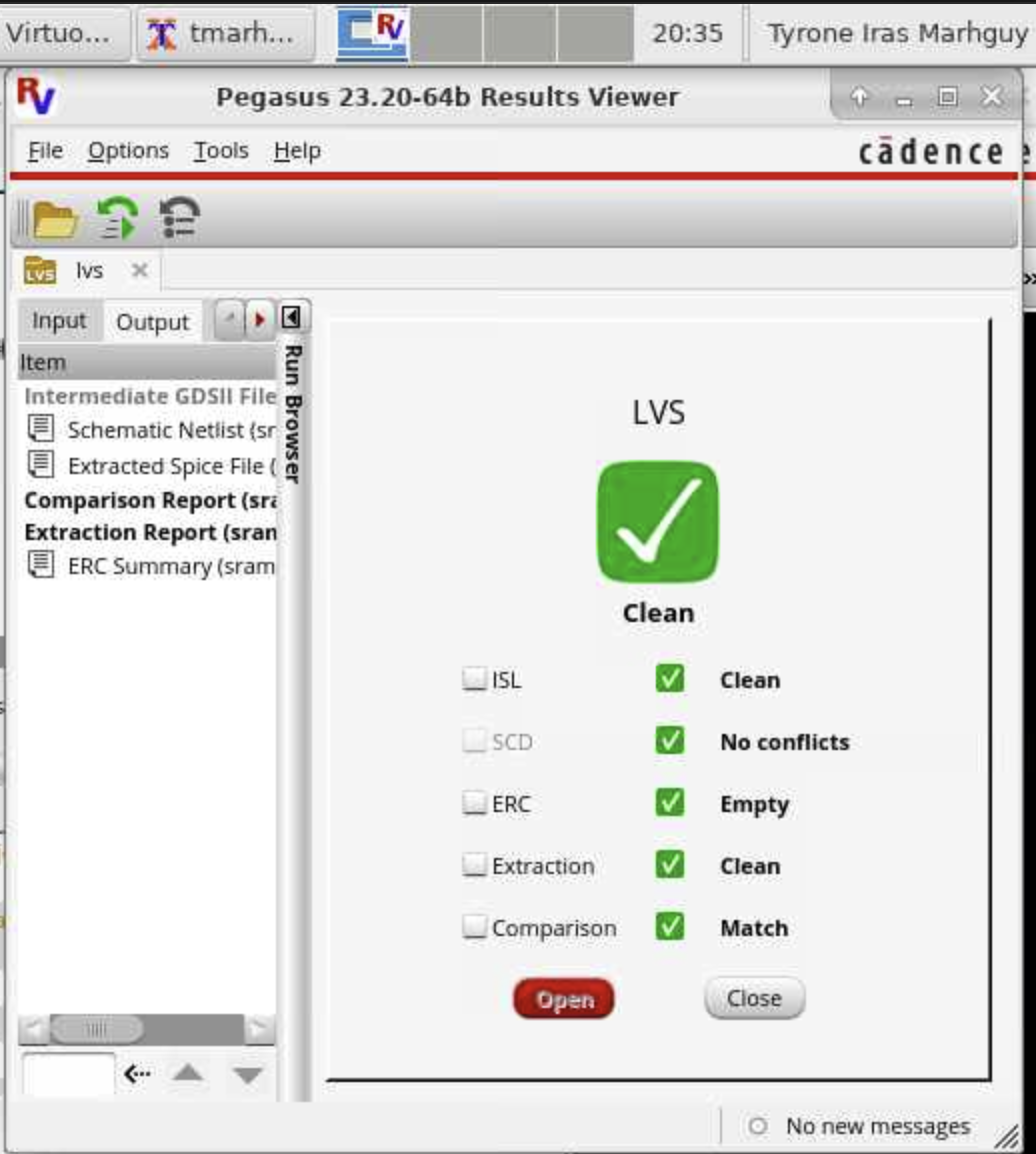
\includegraphics[width=.72\linewidth]{media/part1/current/lvs_clean.png}
\caption{Pegasus 23.20 LVS Results Viewer for Figure~\ref{fig:layout}. The run is clean: ISL clean, SCD with no conflicts, ERC empty, extraction clean, and comparison match.}\label{fig:lvs}
\end{figure}
The area in Table~\ref{tab:area} is the PR-boundary area that abutting cells repeat at; it includes the half-rails and half-bitline-contacts that are shared with the mirrored neighbours, which is the area the Part 2 array actually tiles.

\subsection{Density factor for the area accounting}
The handout estimates un-laid-out blocks as $A_{\rm est}=D\sum_i W_iL_i$ with $D=A_{\rm cell}/\sum_{\rm cell}W_iL_i$ measured from this cell. For FinFETs the drawn width is quantized, so we state the convention: one fin counts as the PDK fin pitch, $W_{\rm fin}=48$ nm (the \texttt{FinArea} grid of \texttt{cds\_ff\_mpt}), and $L=18$ nm for every device. The cell has $4+4+2+2+2+2=16$ fins, so
\begin{equation}
\sum_{\rm cell}W_iL_i=16\times0.048\times0.018\;\mu\mathrm m^2=0.0138\;\mu\mathrm m^2,
\qquad
D=\frac{A_{\rm cell}}{0.0138\;\mu\mathrm m^2}=\densityD .
\label{eq:density}
\end{equation}
The same $W_{\rm fin}$ convention must be used for every $\sum W_iL_i$ in Parts 2 and 3 so that $D$ cancels consistently.

\section{Extraction (handout 1.3)}
Parasitics were extracted from Figure~\ref{fig:layout} with the tutorial Quantus flow (C+CC). Part 2 inherits the per-cell loads:
\begin{table}[H]\centering
\caption{Extracted node capacitance of one cell (WL $=0$, bitlines held at $V_{DD}$ for the DC operating point).}\label{tab:cap}
\begin{tabular}{@{}lll@{}}\toprule
Node & Capacitance & Meaning for Part 2 \\\midrule
BL (one bitline, one cell) & \cBL\ aF & $C_{BL}\approx 16\times$ this $+$ wire per column \\
WL (one cell) & \cWL\ aF & $C_{WL}\approx 4\times$ this $+$ wire per row \\\bottomrule
\end{tabular}
\end{table}
The bitline number is dominated by the pass-gate drain junction plus the shared bitline contact; the wordline number by two pass-gate gate capacitances plus the WL wire across the cell. Fifteen copies of the BL value are the stand-in column load used in the functional check.

\section{Post-layout stability characterization (handout 1.4)}\label{sec:stability}
These benches use the extracted view at $V_{DD}=0.8$ V unless stated. The margin is the same largest-square reduction as Section~\ref{sec:method} (\sourcepath{scripts/check_snm_sweep.py}), and for any asymmetry SNM $=\min(\mathrm{SNM}_L,\mathrm{SNM}_R)$.
\begin{table}[H]\centering
\caption{Post-layout stability results at $V_{DD}=0.8$ V. Setups are the handout's 1.4a--d.}\label{tab:stability}
\begin{tabularx}{\linewidth}{@{}p{.16\linewidth}X p{.2\linewidth}@{}}\toprule
Item & Bench & Result \\\midrule
Hold SNM & WL$=0$; feedback broken; sweep $V_Q$, record $V_{\overline Q}$ and vice versa; overlay. & \snmHold\ mV \\
Read SNM & WL$=V_{DD}$, BL$=$BLB$=V_{DD}$ (ideal sources); same butterfly. & \snmReadPL\ mV \\
Read ``0'' node & DC voltage of the disturbed zero node during the read butterfly; compare to Eq.~\eqref{eq:read-root} and the $77.1$ mV schematic crossing. & \vZeroPL\ mV \\
Write margin & Store $Q=1$; WL$=V_{DD}$; BLB held at $V_{DD}$; sweep BL from $V_{DD}$ to 0; $\mathrm{WM}_{BL}=V_{\rm trip}$. & \wmBL\ V \\
Cell current & WL$=V_{DD}$, both bitlines at $V_{DD}$; current drawn from the zero-side bitline. & \iCell\ $\mu$A \\\bottomrule
\end{tabularx}
\end{table}
\begin{figure}[H]\centering
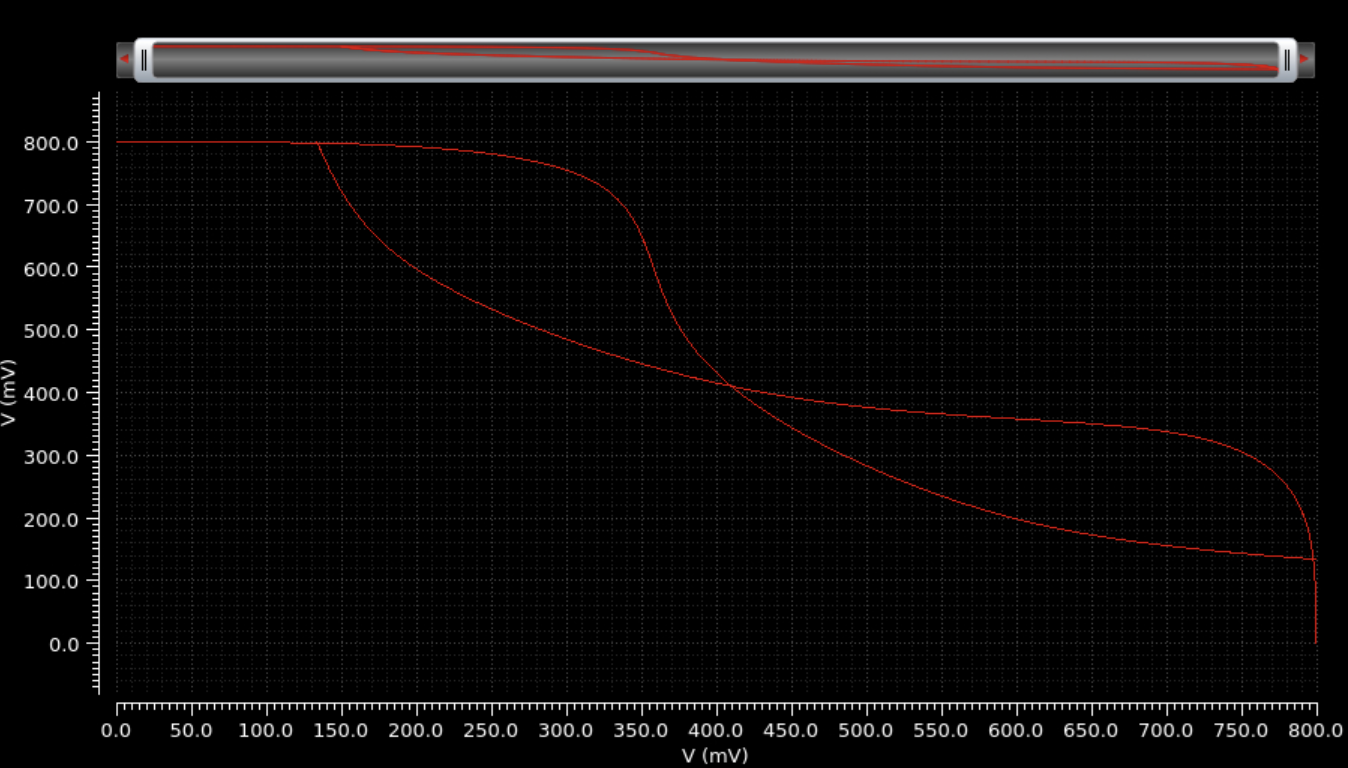
\includegraphics[width=\linewidth]{media/part1/hold_snm_viva.png}
\caption{Hold butterfly at $0.8$ V. WL $=0$, feedback broken, $V_Q$ and $V_{\overline Q}$ overlaid. SNM $=\snmHold$ mV.}\label{fig:pl-butterflies}
\end{figure}

\subsection{Supply dependence (handout 1.4e)}
\begin{table}[H]\centering
\caption{Read SNM and write margin versus supply, extracted view.}\label{tab:supply}
\begin{tabular}{@{}cccc@{}}\toprule
$V_{DD}$ (V) & SNM$_{\rm read}$ (mV) & $\mathrm{WM}_{BL}$ (V) & Comment \\\midrule
0.8 & \snmReadPL & \wmBL & nominal \\
0.7 & \snmReadSeven & \wmSeven & \\
0.5 & \snmReadFive & \wmFive & \worksAtFive \\\bottomrule
\end{tabular}
\end{table}
At the schematic level the $0.8$ V read SNM was $156.3$ mV (Table~\ref{tab:sweep}). Extraction lowers that to \snmReadPL\ mV and raises the disturbed zero node from $77.1$ mV to \vZeroPL\ mV. Read SNM falls further to \snmReadSeven\ mV at $0.7$ V and \snmReadFive\ mV at $0.5$ V, while $\mathrm{WM}_{BL}$ falls from \wmBL\ V to \wmSeven\ V and then \wmFive\ V. At $0.5$ V the cell still reads, and a full write still completes. $\mathrm{WM}_{BL}=$ \wmFive\ V is the smallest margin in the table, so the write is the weak result.

\section{Functional check (handout 1.5)}\label{sec:functional}
The transient bench drives WL and the precharge devices with ideal pulses and loads each bitline with the extracted cell plus 15 copies of the per-cell bitline capacitance from Table~\ref{tab:cap}, standing in for the 16-row Part 2 column. The sequence is write 0, read, write 1, read. Both writes finish inside the WL pulse, and both reads leave $Q$ and $\overline Q$ in place.

\section{What limits the cell, and what changes for Part 2}
Read stability is set by the pass-gate/pull-down divider. The schematic sweep moved the disturbed zero node from $134$ mV ($\beta=1$) to $77$ mV ($\beta=2$) and raised read SNM by $30$ mV. Extraction gives \snmReadPL\ mV of read SNM and a \vZeroPL\ mV zero node at $0.8$ V, against a hold SNM of \snmHold\ mV, so the read is what the Part 2 noise budget has to clear. The cost of $\beta=2$ is the four-fin pull-down, which sets the \cellH\ $\mu$m cell height and most of $C_{WL}=$ \cWL\ aF, and the two-fin pass-gate, which sets $C_{BL}=$ \cBL\ aF and the \iCell\ $\mu$A read current the sense path integrates. Writability is the $\gamma=1$ limit: $\mathrm{WM}_{BL}$ is \wmBL\ V at $0.8$ V and only \wmFive\ V at $0.5$ V. The cell still reads at $0.5$ V (\snmReadFive\ mV), and a full write still completes. The write is the weak one, so a Part 2 remedy, if that margin is not enough for the column, is a weaker pull-up or a write assist rather than a new cell. Part 2 keeps this cell, mirrors it to share the BL contacts and the VDD/VSS rails, and sizes the wordline driver and precharge from $16\times$ \cBL\ aF and $4\times$ \cWL\ aF plus wire.

\section*{Traceability and team contributions}
The handout used for this report is \sourcepath{docs/ese5700-project1.pdf} (Part 1 on pp.~3--4). Reproducible results are in \sourcepath{results/part1/read-snm/beta1/}, \sourcepath{beta1p5/}, and \sourcepath{beta2/}; each contains \sourcepath{raw.csv}, normalized curves and \sourcepath{snm.json}. The overlay coordinates are the two \sourcepath{lobes} entries in those JSON files. Recompute with the command below. The original handwritten and Cadence images are retained in \sourcepath{media/part1/}.

\begin{center}\small\texttt{python3 scripts/check\_snm\_sweep.py --all}\end{center}

The selected design was also captured in separate $Q$- and $\overline Q$-side sweep schematics (Figure~\ref{fig:variants}). They show the symmetric device assignment used by the transfer-curve benches. The layout itself is Figure~\ref{fig:layout}.
\begin{figure}[H]\centering
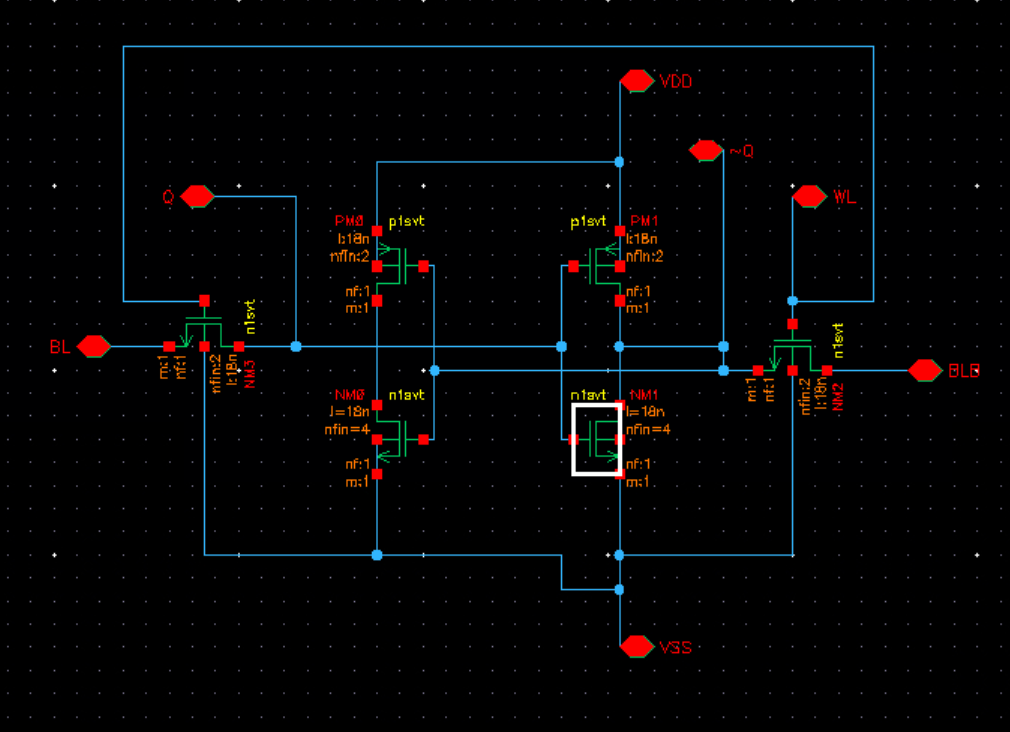
\includegraphics[width=.98\linewidth,height=.30\textheight,keepaspectratio]{media/part1/read_snm_q_sch_2.png}
\caption{Original Cadence $Q$-side cell for $\beta=2$.}\label{fig:variants}
\end{figure}
\begin{figure}[H]\centering
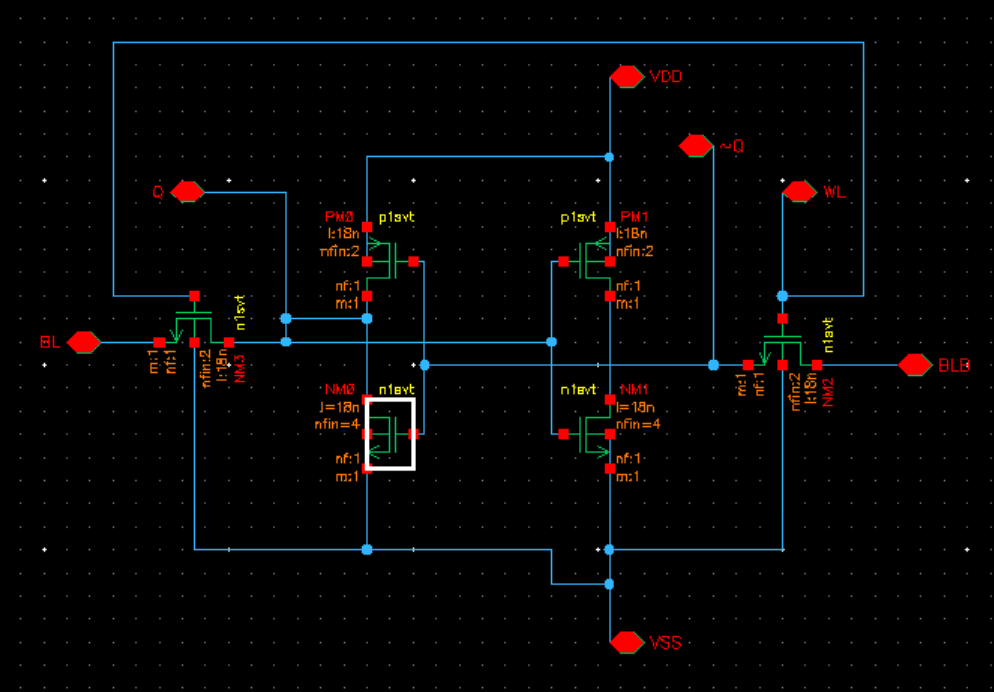
\includegraphics[width=.98\linewidth,height=.30\textheight,keepaspectratio]{media/part1/read_snm_qb_sch_2.png}
\caption{Original Cadence $\overline Q$-side cell for $\beta=2$. The other PD variants remain in \sourcepath{media/part1/}.}
\end{figure}

\begin{table}[H]\centering\small
\caption{Team contributions (handout requirement). Both authors are responsible for understanding the complete design and report.}\label{tab:contrib}
\begin{tabularx}{\linewidth}{@{}p{.28\linewidth}X@{}}\toprule
Tyrone Marhguy & Schematic, hand read analysis, three-point $\beta$ sweep, custom layout, Pegasus LVS, and report assembly. \\
Victor Wanjohi & Hand write analysis, extraction, post-layout stability, and the functional check. \\\bottomrule
\end{tabularx}
\end{table}
Both authors are responsible for the complete design and for every result in this report.
\end{document}
